\documentclass[12pt, a4paper]{article}
\usepackage[czech]{babel}

\usepackage{graphicx}
\usepackage{parskip}
\usepackage{longtable}
\usepackage{amsmath}
\usepackage{float}
\usepackage{url}

\usepackage[backend=biber,style=authoryear]{biblatex}
\addbibresource{zdroje.bib}

\begin{document}

\begin{titlepage}
    \centering
    {\large UNIVERZITA KARLOVA\par}
    \vspace{0.2cm}
    {\large {Přírodovědecká fakulta}\par}
    \vspace{0.2cm}
    {\large Katedra aplikované geoinformatiky a kartografie\par}

    \vspace{2cm}

    {\large Studijní program:\par}
    \vspace{0.2cm}
    {\large Geoinformatika, kartografie a dálkový průzkum Země\par}

    \vspace{2cm}

    
\includegraphics[width=5cm]{logo.png}\par

    \vspace{1cm}

    {\large \textbf{Jakub Fuchsig, Šimon Kohout}\par}
    \vspace{1cm}
    {\Large \textbf{Generalizace budov LOD0}\par}
    \vspace{2cm}  
    {\large Ústí nad Labem, Zákupy 2026\par} 
\end{titlepage}

\section{Zadání}

Vstup: množina budov $B = \{B_i\}_{i=1}^n$, budova $B_i = \{P_{i,j}\}_{j=1}^m$.

Výstup: $G(B_i)$.

Ze souboru načtěte vstupní data představovaná lomovými body budov a proveďte generalizaci budov do úrovně detailu LOD0. Pro tyto účely použijte vhodnou datovou sadu, např. ZABAGED, testování proveďte nad třemi datovými sadami (historické centrum města, sídliště, izolovaná zástavba).

Pro každou budovu určete její hlavní směry metodami:

\begin{itemize}
    \item Minimum Area Enclosing Rectangle,
    \item PCA.
\end{itemize}

U první metody použijte některý z algoritmů pro konstrukci konvexní obálky. Budovu při generalizaci do úrovně LOD0 nahraďte obdélníkem orientovaným v obou hlavních směrech, se středem v těžišti budovy, jeho plocha bude stejná jako plocha budovy. Výsledky generalizace vhodně vizualizujte.

Otestujte a porovnejte efektivitu obou metod s využitím hodnotících kritérií. Pokuste se rozhodnout, pro které tvary budov dávají metody nevhodné výsledky, a pro které naopak poskytují vhodnou aproximaci.

\section{Zpracované bonusové úlohy}

Pro tuto úlohu byly zpracovány níže vypsané úlohy společně s jejich ohodnocením.



\begin{small}
\begin{longtable}{|p{12cm}|c|}
    \hline
    \textbf{Krok} & \textbf{Hodnocení} \\
    \hline
    \endfirsthead
    
    \hline
    \textbf{Krok} & \textbf{Hodnocení} \\
    \hline
    \endhead

    Generalizace budov metodami Minimum Area Enclosing Rectangle a PCA. & 15b \\
    \hline
    \textit{Generalizace budov metodou Longest Edge.} & +5b \\
    \hline
    \textit{Generalizace budov metodou Wall Average.} & +8b \\
    \hline
    \textit{Generalizace budov metodou Weighted Bisector.} & +10b \\
    \hline
    \textit{Ošetření singulárních případů při generování konvexní obálky.} & +2b \\
    \hline
    \textit{Načtení vstupních dat ze *.shp.} & +10b \\
    \hline
    \textbf{Celkem splněno:} & \textbf{50b} \\
    \hline
\end{longtable}
\end{small}


\section{Úvod}
Různá měřítka map zobrazují různé oblasti s odlišnými přiblíženími. Důležitým krokem při změně měřítka je rozhodnutí, jak budou některé mapové prvky zobrazeny v mapě. Tento proces se nazývá generalizace a je jedním z nejdůležitějších kroků při tvorbě mapového díla. Cílem tohoto procesu je zachování přibližného tvaru, orientace či plochy prvku.

Pro tuto úlohu byly generalizovány budovy do podoby detailu LOD0, tedy původní půdorys budovy se nahradí jednoduchým geometrickým tvarem, nejčastěji obdélníkem. Proces generalizace byl prováděn metodami, které se snaží zachovat orientaci, plochu a velikost původní budovy. Použitými metodami jsou \textit{Minimum Area Enclosing Rectangle (MBR)}, \textit{Principal Component Analysis (PCA)}, \textit{Longest Edge}, \textit{Wall Average} a \textit{Weighted Bisector}, které tyto požadavky splňují, přestože každá metoda přistupuje k určování, zejm. hlavních směrů, jinak.

Pro testování na reálných datech byly metody aplikovány na třech typech zástavby:
\begin{itemize}
    \item \textbf{historické centrum města} - pro tuto zástavbu bylo zvoleno centrum města Česká Lípa
    \item \textbf{sídliště} - vzorkem této zástavby se stalo sídliště Severní terasa v Ústí nad Labem
    \item \textbf{izolovaná zástavba} - jedná se o budovy, zejm. rodinné domky, z vesnice Božíkov u města Zákupy
\end{itemize}

\section{Konvexní obálka}
Konvexní obálka (ang. \textit{convex hull - ch}) je jedna z nejpoužívanějších geometrických struktur nejen kartografické generalizace. Jedná se o konvexní mnohoúhelník, který obsahuje veškeré body a jehož plocha je nejmenší možná. Tuto obálku lze často využít např. ke konstrukci \textit{Minimum Bounding Rectangle (MBR)}, který se právě využívá v kartografické generalizaci pro zjištění tvaru a orientace budov.


\subsection{Konstrukce konvexní obálky}
Ke konstrukci tohoto konvexního mnohouhelníku lze přistupovat vícero metodami. Nejčastěji je možné se setkat s metodou \textbf{\textit{Jarvis Scan}}, který byl použit v tomto úkolu, a s metodou \textbf{\textit{Graham Scan}}.

\subsubsection{Jarvis Scan}
Jedná se o velmi intuitivní přístup konstrukce konvexní obálky. Metoda funguje na principu maximalizace vnitřního úhlu k hledaným bodům. V každém kroku je tedy hledán nový bod, který svírá s aktuální hranou největší úhel - tudíž se jedná o hranici množiny. Důležitým předpokladem je, že metoda je iniciována v bodě s nejmenší Y-ovou (případně X-ovou) souřadnicí. Nevýhodou je jeho časová složitost ve velkých množinách, jelikož prochází v každém kroku všechny body.

Níže je zobrazen princip algoritmu \textit{Jarvis Scan}.

\begin{figure}[H]
    \centering
    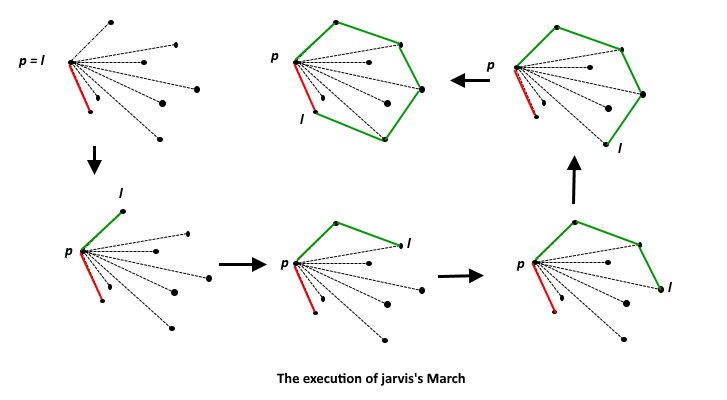
\includegraphics[width=1\textwidth]{JarvisAlgorithm.png}
    \caption{Princip algoritmu Jarvis Scan \parencite{Jarvis}}
\end{figure}

\subsubsection{Graham Scan}
Tento algoritmus nebyl v této práci využit, přestože je to efektivnější přístup. Jeho nevýhodou však je, že ho není možné použít pro 3D data. Pro tuto metodu je opět nutné zvolení počátečního bodu, od kterého jsou následně počítány úhly ke zbývajícím bodům a ty se následně seřadí. Body se následně cyklicky procházejí a pokud spadají do \textbf{levé} poloroviny, stávají se součástí obálky, pokud náleží \textbf{pravé} polorovině, jsou z obálky odebrány.

\section{Použité algoritmy}
\subsection{Algoritmus \textit{Minimum Area Enclosing Rectangle}}
Tento algoritmus je založen na mětodě hledání opsaného obdélníku s minimální plochou. Vychází z teoretického
předpokladu, že alespoň jedna strana takového obdélníku musí být kolineární s hranou
konvexní obálky objektu. Proces zahrnuje nejprve konstrukci konstrukci konvexní obálky, poté natočení obálky tak, aby jejejí hrana byla rovnoběžná s osou x (úhel $-sigma$). Dále je nutné najít její minimální a maximální souřadnice x a y, z nichž se dále vytvoří \textit{min-max box}. Po výpočtu plochy a nalezení nejmenšího boxu je posléze zpět natočet o úhel $sigma$ do původní orientace \parencite{bayer}.

V naší implementaci je proces nalezení tohoto obdélníku obsažen ve funkci \texttt{createMBR} a jeho finální úprava ve funkci \texttt{simplifyBuildingMBR}. Metoda využívá následující kroky:

\begin{enumerate}
    \item \textbf{Konstrukce konvexní obálky:} Z polygonu původní budovy se pomocí funkce \texttt{createCH} (Jarvis Scan) vytvoří konvexní obálka \texttt{ch}.
    \item \textbf{Inicializace minima:} Pro počáteční porovnávání se nad obálkou \texttt{ch} vytvoří základní min-max box \texttt{mmb\_min} a pomocí funkce \texttt{createMMB} se vypočte jeho plocha \texttt{area\_min}.
    \item \textbf{Iterace a rotace obálky:} Algoritmus v cyklu prochází všechny hrany obálky. Pro každou hranu se z rozdílu souřadnic koncových bodů (\texttt{dx}, \texttt{dy}) vypočte její směrový úhel \texttt{sigma} (pomocí funkce \texttt{atan2}). Obálka se následně pomocí \texttt{rotatePolygon} natočí o úhel \texttt{-sigma} tak, aby daná hrana ležela rovnoběžně s osou $x$ (vznikne rotovaná obálka \texttt{ch\_r}).
    \item \textbf{Určení aktuálního min-max boxu:} Nad rotovanou obálkou \texttt{ch\_r} se opět zavolá funkce \texttt{createMMB}, která nalezne aktuální ohraničující obdélník \texttt{mmb} a vypočte jeho plochu \texttt{area}.
    \item \textbf{Aktualizace minima:} Je-li aktuální plocha \texttt{area} menší než dosud nejmenší známá plocha \texttt{area\_min}, hodnoty se aktualizují: uloží se nová minimální plocha, \texttt{mmb\_min = mmb} a zapamatuje se nejlepší úhel natočení \texttt{sigma\_min = sigma}.
    \item \textbf{Zpětná rotace a upravení velikosti:} Nejmenší nalezený min-max box \texttt{mmb\_min} se natočí zpět o úhel \texttt{sigma\_min}, čímž vznikne obdélník \texttt{mbr} orientovaný ve směru budovy. Finálně se zavolá funkce \texttt{resizeRectangle}, která velikost tohoto obdélníku od jeho středu proporčně upraví (\texttt{mbr\_res}) tak, aby jeho výsledná plocha přesně odpovídala ploše původní budovy.
\end{enumerate}

\subsection{Algoritmus \textit{Principal Component Analysis}}
Metoda PCA určuje hlavní směry budovy na základě rozptylu jejích bodů. Matematickým základem je singulární rozklad (SVD) kovarianční matice souřadnic bodů budovy. Vlastní vektory získané tímto rozkladem definují osy, ve kterých má objekt největší a nejmenší variabilitu, což odpovídá jeho hlavním směrům. Metoda je velmi rychlá, avšak může vykazovat nižší efektivitu u pravidelných objektů, jako je čtverec nebo kružnice \parencite{bayer}.

V naší implementaci je proces generalizace metodou PCA obsažen ve funkci \texttt{simplifyBuildingPCA}. Metoda využívá následující kroky:

\begin{enumerate}
    \item \textbf{Zisk souřadnic:} Z polygonu původní budovy se iterací přes všechny její lomové body oddělí souřadnice do samostatných seznamů \texttt{X} a \texttt{Y}. Z těchto seznamů se následně pomocí knihovny \textit{NumPy} vytvoří dvourozměrná matice souřadnic \texttt{A}.
    \item \textbf{Výpočet kovarianční matice:} Z matice \texttt{A} se pomocí funkce \texttt{np.cov} vypočítá kovarianční matice \texttt{C}.
    \item \textbf{Dekompozice matice (SVD):} Na kovarianční matici \texttt{C} je aplikován rozklad singulárních hodnot pomocí funkce \texttt{np2.svd}. Operace vrací tři matice: \texttt{U}, \texttt{S} a \texttt{V}, kde matice \texttt{V} představuje směrové vektory hlavních komponent.
    \item \textbf{Určení hlavního směru:} K získání hlavního úhlu budovy \texttt{sigma} se použije první vektor z matice \texttt{V} (prvky \texttt{V[0][0]} a \texttt{V[0][1]}), který reprezentuje směr s největším rozptylem a aplikací funkce \texttt{atan2}.
    \item \textbf{Rotace a min-max box:} Polygon původní budovy se pomocí funkce \texttt{rotatePolygon} natočí o úhel \texttt{-sigma} tak, aby byl jeho hlavní směr rovnoběžný s osou $x$ (vznikne rotovaná budova \texttt{build\_rot}). Nad tímto polygonem se následně zavolá funkce \texttt{createMMB}, která vytvoří ohraničující \textit{min-max box} \texttt{mmb}.
    \item \textbf{Zpětná rotace a upravení velikosti:} Min-max box \texttt{mmb} se pomocí \texttt{rotatePolygon} natočí zpět o úhel \texttt{sigma}, čímž vznikne obdélník \texttt{mbr} orientovaný podle hlavního směru budovy. Finálně se využije funkce \texttt{resizeRectangle}, která upraví velikost tohoto obdélníku(\texttt{mbr\_res}) tak, aby jeho plocha odpovídala ploše původní budovy.
\end{enumerate}

\subsection{Algoritmus \textit{Longest Edge}}
Tato metoda z předpokládá, že nejdelší dostupná hrana polygonu udává primární směr celé budovy. Algoritmus tedy prochází všechny stěny, nalezne tu s maximální délkou a vypočítá její úhel. Získaná orientace se následně využije pro pootočení původního polygonu tak, aby se kolem něj dal zkonstruovat obdélník s minimální plochou (min-max box). Ačkoliv je metoda algoritmicky i výpočetně velmi jednoduchá, u složitějších nepravidelných tvarů budov nemusí vždy nejdelší hrana reprezentovat kartograficky nejvhodnější celkový směr \parencite{bayer}.

V naší implementaci je tento postup obsažen ve funkci \texttt{simplifyBuildingLongestEdge}. Metoda využívá následující kroky:

\begin{enumerate}
    \item \textbf{Procházení hran:} Pomocí cyklu se iteruje přes všechny hrany polygonu budovy. Pro každou hranu se určí rozdíl souřadnic jejích koncových bodů (\texttt{dx}, \texttt{dy}) a pomocí Pythagorovy věty se vypočítá její délka \texttt{length}.
    \item \textbf{Nalezení maxima a určení směru:} Pokud je vypočtená délka hrany větší než dosavadní zaznamenané maximum (\texttt{max\_length}), hodnoty se aktualizují. Nová délka se uloží jako největší a pomocí funkce \texttt{atan2} se z rozdílů souřadnic (\texttt{dy}, \texttt{dx}) vypočítá její směrový úhel, který se uloží do proměnné \texttt{best\_angle}.
    \item \textbf{Opakující se kroky naší generalizace:} Jakmile je iterace dokončena a je určen hlavní úhel budovy (\texttt{best\_angle}), provedou se výše zmíněné kroky pro vytvoření a úpravu obdélníku, které jsou identické pro všechny implementované metody:
    \begin{itemize}
        \item Pomocí \texttt{rotatePolygon} se budova natočí o úhel \texttt{-best\_angle}.
        \item Funkcí \texttt{createMMB} se nad natočenou budovou vytvoří \textit{min-max box} (\texttt{mmb}).
        \item Tento box se natočí zpět o úhel \texttt{best\_angle} do reálné orientace (\texttt{mbr}).
        \item Funkce \texttt{resizeRectangle} proporčně upraví velikost obdélníku k těžišti tak, aby jeho plocha odpovídala původní budově (\texttt{mbr\_res}).
    \end{itemize}
\end{enumerate}


\subsection{Algoritmus \textit{Wall Average}}
Alternativou k metodě nejdelší hrany je metoda váženého průměru stěn \textit{Wall Average}, která pro určení orientace využívá informace o všech hranách budovy. Algoritmus vychází z předpokladu, že typické struktury budov jsou tvořeny primárně pravoúhlými stěnami. Získané úhly jednotlivých stěn jsou proto převedeny do prvního kvadrantu pomocí zbytku po dělení (modulo) $pi/2$. Výsledný orientační směr budovy je pak určen jako průměr takto upravených úhlů, avšak s uplatněním délek jednotlivých stěn coby vah. Nejsilněji tedy výslednou orientaci ovlivňují ty nejdelší stěny, zatímco vliv drobných rohů a výstupků je minimalizován \parencite{bayer}.

V naší implementaci je tento postup obsažen ve funkci \texttt{simplifyBuildingWallAverage}. Metoda využívá následující kroky:

\begin{enumerate}
    \item \textbf{Výpočet délek a úhlů:} Algoritmus iteruje přes všechny hrany polygonu. Pro každou hranu se z rozdílu souřadnic (\texttt{dx}, \texttt{dy}) vypočte její délka (\texttt{length}) a její směrový úhel (\texttt{angle}) pomocí funkce \texttt{atan2}.
    \item \textbf{Sjednocení orientace:} Pro sjednocení orientace vzájemně kolmých stěn se na vypočtený úhel aplikuje operace modulo $\pi/2$ (\texttt{angle \% (pi/2)}).
    \item \textbf{Aplikace vah:} Průběžně se sčítají celkové délky všech obvodových hran (\texttt{sum\_lenghts}) a zároveň i součiny redukovaných úhlů s délkou dané hrany (\texttt{sum\_angles\_lenghts}). 
    \item \textbf{Výpočet váženého průměru:} Výsledný hlavní úhel budovy (\texttt{best\_angle}) je následně vypočítán jako podíl sumy vážených úhlů a sumy délek.
    \item \textbf{Opakující se kroky naší generalizace:} Se zjištěným hlavním úhlem se provedou totožné kroky tvorby obdélníku jako u ostatních metod:
    \begin{itemize}
        \item Natočení polygonu budovy o úhel \texttt{-best\_angle} (funkce \texttt{rotatePolygon}).
        \item Vytvoření ohraničujícího \textit{min-max boxu} (funkce \texttt{createMMB}).
        \item Zpětná rotace obdélníku o úhel \texttt{best\_angle}.
        \item Proporční úprava plochy výsledného obdélníku tak, aby odpovídala ploše budovy (funkce \texttt{resizeRectangle}).
    \end{itemize}
\end{enumerate}

\subsection{Algoritmus \textit{Weighted Bisector}}
Tento algoritmus přistupuje k hledání hlavní orientace budovy odlišným způsobem než předchozí metody. Namísto analýzy hran mnohouhelníku zkoumá diagonály mezi všemi vrcholy polygonu. Konkrétně vybírá dvě nejdelší různoběžné diagonály a výsledný orientační směr počítá jako jejich vážený průměr, přičemž jako váhy slouží právě délky těchto diagonál. Tím je zajištěno, že nejdelší osa budovy má na výsledek největší vliv \parencite{bayer}.

V naší implementaci je tento postup obsažen ve funkci \texttt{simplifyBuildingWB}. Metoda využívá následující kroky:

\begin{enumerate}
    \item \textbf{Generování diagonál:} Pomocí dvou cyklů se iteruje přes všechny dvojice nesousedních vrcholových bodů budovy. Pro každou platnou dvojici se z rozdílů souřadnic (\texttt{dx}, \texttt{dy}) vypočítá délka spojnice (\texttt{s}) a její směrový úhel (\texttt{sigma}). Úhel se následně redukuje do intervalu $<0, \pi>$ a obě hodnoty se uloží do seznamu \texttt{diagonals}.
    \item \textbf{Výběr primární diagonály:} Seznam vytvořených diagonál se seřadí sestupně podle jejich délky. První prvek seznamu je označen jako absolutně nejdelší diagonála s parametry délky \texttt{s1} a směrnice \texttt{sigma1}.
    \item \textbf{Výběr sekundární diagonály:} Algoritmus dále prochází seřazený seznam a hledá druhou nejdelší diagonálu (\texttt{s\_cand}, \texttt{sigma\_cand}). Využívá přitom kontrolní podmínku: úhlový rozdíl (\texttt{diff}) mezi kandidátem a primární diagonálou musí být větší než námi stanovená tolerance (\texttt{angle\_tolerance} = $10°$). Tím je zajištěno, že vybraná sekundární diagonála (\texttt{s2}, \texttt{sigma2}) není s tou primární rovnoběžná.
    \item \textbf{Výpočet váženého směru:} Před samotným výpočtem průměru proběhne korekce úhlů, aby obě úsečky směřovaly do stejné poloroviny (rozdíl úhlů menší než $\pi/2$). Následně se vypočte výsledný orientační směr budovy (\texttt{sigma\_weight}) podle rovnice váženého průměru: 
    
    $$\sigma_{weight} = \frac{s_1 \cdot \sigma_1 + s_2 \cdot \sigma_2}{s_1 + s_2}$$

    
    \item \textbf{Opakující se kroky naší generalizace:} S vypočteným úhlem \texttt{sigma\_weight} se provedou totožné kroky tvorby obdélníku jako u ostatních metod:
    \begin{itemize}
        \item Natočení polygonu budovy o úhel \texttt{-sigma\_weight} (funkce \texttt{rotatePolygon}).
        \item Vytvoření ohraničujícího \textit{min-max boxu} (funkce \texttt{createMMB}).
        \item Zpětná rotace obdélníku o úhel \texttt{sigma\_weight}.
        \item Proporční úprava plochy výsledného obdélníku tak, aby odpovídala ploše budovy (funkce \texttt{resizeRectangle}).
    \end{itemize}
\end{enumerate}

\section{Ošetření singulárních případů}
Tento bonusový úkol byl tvořen pro metodu tvorby konvexní obálky (\textit{Jarvis Scan}), která je v naší implementaci řešena ve funkci \texttt{createCH} uvnitř třídy \texttt{Algorithms}. Bylo nutné ošetřit některé singulární případy, které se mohou v datech vyskytnout a způsobit pád aplikace nebo chybné vykreslení tvaru:

\begin{itemize}
    \item \textbf{Nedostatečný počet bodů:} Zásadním krokem je kontrola vstupu. Pokud má vstupní množina bodů (polygon \texttt{pol}) méně než 3 vrcholy (\texttt{len(pol) < 3}), není možné konvexní obálku vytvořit a algoritmus by měl tyto body rovnou vrátit beze změn a bez dalšího výpočtu.
    
    \item \textbf{Inicializační vektor a prevence dělení nulou:} Algoritmus začíná od nejnižšího bodu (pivota \texttt{q}) a potřebuje referenční linii pro start měření úhlů k dalším bodům. Pokud by byl jako startovní pomocný bod zvolen bod se stejnými souřadnicemi jako pivot, vznikne vektor o nulové délce a výpočet ve funkci \texttt{get2VectorsAngle} spadne kvůli dělení nulou. Řešením je vytvoření umělého bodu \texttt{pj1} odsunutého po ose X vlevo od pivota s využitím třídy \texttt{QPointF(q.x() - 100, q.y())}, což zaručí vznik validního počátečního horizontálního vektoru.
    
    \item \textbf{Kolineární body:} Speciálním úkazem jsou body ležící na stejné přímce. V algoritmu to znamená, že testovaný kandidát svírá se současným vrcholem obálky identický úhel jako dosud nejlepší nalezený bod (\texttt{omega == omega\_max}). Řešení spočívá ve výpočtu a porovnání druhé mocniny vzdáleností obou bodů od aktuálního vrcholu (\texttt{dist\_max} a \texttt{dist\_i}). Algoritmus ignoruje bližší body a aktualizuje index \texttt{index\_max} pouze ve chvíli, kdy kandidát leží na přímce nejdále (\texttt{dist\_i > dist\_max}).
\end{itemize}

Pro úpravu některých částí kódu, zejm. syntaxe a chyb, byl použit nástroj AI. Tyto části kódu byly označeny komentáři, ve kterých je podrobněji popsáno, k čemu byla AI využita. Dále byla AI použita k nastínění postupu při tvorbě skriptu např. v hodnocení přesnosti (viz níže).

\section{Popis aplikace}
Pro generalizaci budov do úrovně detailu LOD0 byla vytvořena kostra aplikace v \textit{QT Designer}, která byla dále upravena do výsledné podoby (obrázek2). Uživatel má možnost ručního kreslení polygonu pomocí klikání myši v okně či může zvolit možnost nahrání vlastního souboru \textit{.shp} pomocí tlačítka \textit{File -$>$ Open} či ikonky složky.


\begin{figure}[H]
    \centering
    
\includegraphics[width=1\textwidth]{aplikace.png}
    \caption{Okno aplikace s ručně vytvořeným polygonem}
\end{figure}

Pro generalizaci budovy si uživatel může zvolit z výše zmíněných algoritmů pomocí výběru ikonky z horní lišty. Po stisknutí zvolené ikonky proběhne výpočet generalizace a v okně se vykreslí červený obdélník pro každou budovu, který značí zjednodušený tvar (obrázek 3). Dále se také objeví vyskakovací okno s informacemi o použité metodě a její přesnosti (viz níže).

\begin{figure}[H]
    \centering
    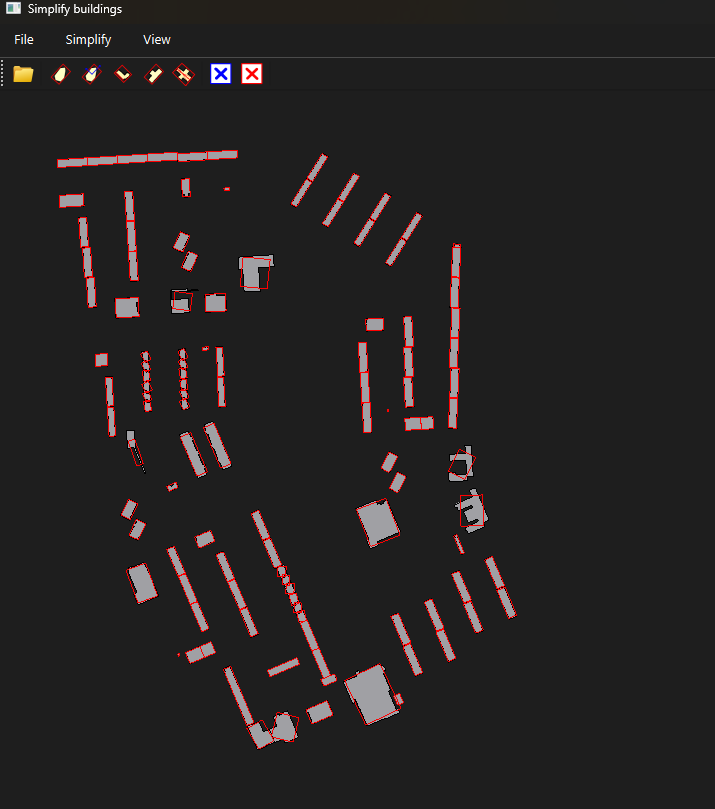
\includegraphics[width=1\textwidth]{generalizace_usti.png}
    \caption{Generalizace sídliště Severní terasa pomocí algoritmu \textit{Weighted Bisector}}
\end{figure}

\textbf{Výstupem} aplikace je kartografická generalizace polygonů v podobě jednoduchý obdélníků (LOD0), které mají stejnou plochu jako původní polygony a podrobný výpis přesnosti použité metody generalizace společně s výpisem počtu "správně" zjednodušených budov (obrázek 4).

\begin{figure}[H]
    \centering
    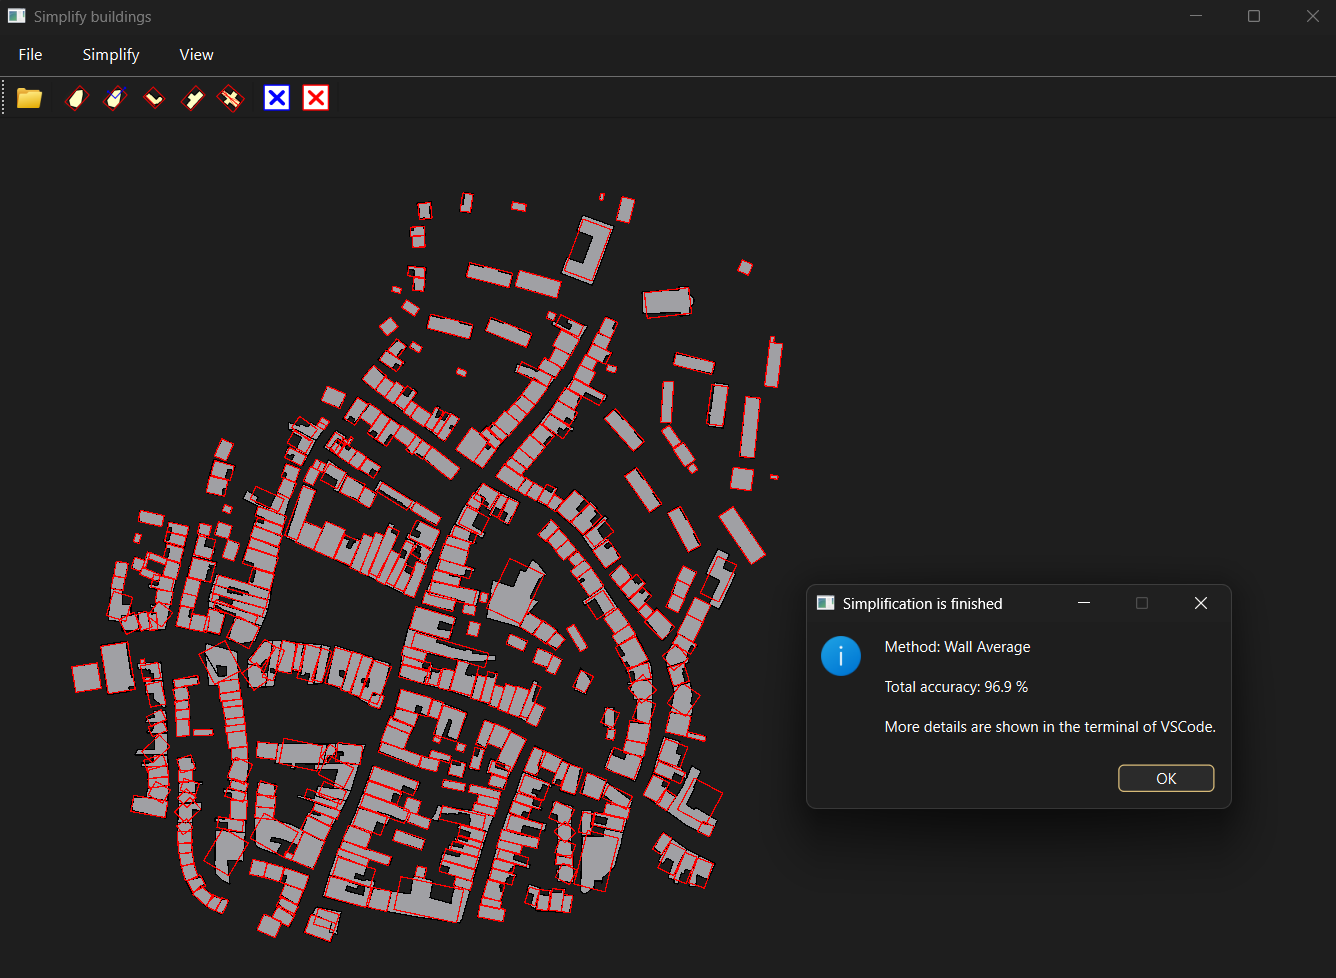
\includegraphics[width=1\textwidth]{vyskakovaci_okno.png}
    \caption{Ukázka vyskakovacího okna s detaily generalizace}
\end{figure}


\section{Hodnocení přesnosti}
Jelikož jednotlivé metody generalizace fungují na lehce odlišných principech, lze očekávat, že jejich přesnost bude různá. Pro otestování a výpočet přesností byly jednotlivé metody použity na třech datasetech, které měly charakteristické půdorysy budov. První dataset je sídliště Severní terasa v Ústí n. Labem, ve které jsou především panelové domy, které mají většinou jednoduchý obdélníkový půdorys. Dataset sídliště obsahoval 113 budov. 

Druhým datasetem je historické centrum v České Lípě, které je naopak charakteristické svými nepravidelnými a složitými půdorysy budov. Tento dataset obsahoval 418 budov.

Třetím datasetem je izolovaná vesnická zástavba obce Zákupy - Božíkov, ve které se objevují převážně izolované rodinné domy či chalupy. Tento dataset lze označit za komplexní, jelikož se zde objevují jak jednoduché tak i složitější půdorysy budov a obsahoval 107.

Výpočet byl prováděn pro jednotlivé budovy, za předpokladu, že jsou min-max boxy pravoúhlé. Pro výpočet byla použita střední hodnota čtverců úhlových odchylek jednotlivých segmentů :

$$\Delta\sigma = \frac{\pi}{2n} \cdot \sqrt{\sum_{i=1}^{n} (r_i - \overline{r})^2}
$$

kde byla zvolena hranice pro určení správnosti a akceptaci objektů hranice $\Delta\sigma < 10^{\circ}$ \parencite{bayer}.

Pro dataset sídliště, který obsahoval jednoduché půdorysy budov vyšly výsledky hodnocení přesnosti velice dobře. V tabulce 2, kde jsou zobrazené výsledky pro jednotlivé metody lze pozorovat, že se přesnosti pohybují nad 98 \% u všech metod. Vysoká přesnost u tohoto datasetu je důsledkem velice jednoduchých půdorysů a tedy generalizace byla relativně jednoduchá. Díky tomu skoro všechny polygony LOD0 splňovaly výše zmíněnou podmínku $10^{\circ}$.
%usti presnost
\begin{small}
\begin{longtable}{|l|c|c|c|}
    \hline
    & \multicolumn{3}{c|}{\textbf{sídliště (Ústí n. Labem)}} \\
    \hline
    \textbf{Metoda} & \textbf{Počet budov} & \textbf{Správně} & \textbf{Přesnost [\%]} \\
    \hline
    \endfirsthead
    
    \hline
    & \multicolumn{3}{c|}{\textbf{sídliště (Ústí n. Labem)}} \\
    \hline
    \textbf{Metoda} & \textbf{Počet budov} & \textbf{Správně} & \textbf{Přesnost [\%]} \\
    \hline
    \endhead

    \textit{MBR} & 113 & 111 & 98.2 \\
    \hline
    \textit{PCA} & 113 & 110 & 97.3 \\
    \hline
    \textit{Longest Edge} & 113 & 111 & 98.2 \\
    \hline
    \textit{Wall Avergae} & 113 & 111 & 98.2 \\
    \hline
    \textit{Weighted Bisector} & 113 & 111 & 98.2 \\
    \hline
    \caption{Hodnocení generalizace - sídliště}
    
\end{longtable}
\end{small}
Dosti odlišným případem byl dataset historického centra v České Lípě. Z výsledků přesnosti zde vyčnívá metoda \textbf{PCA}, která dosahovala výrazně nižší přesnosti než zbylé metody (tabulka 3). Jelikož dataset obsahuje složité budovy, metoda PCA stěží určovala hlavní směry budovy a tudíž se nesplnila podmínka akceptace. Dále lze v tabulce 3 pozorovat, že se lehce snížila přesnost i ostatních metod na asi 96 \%. K poklesu mohlo dojít i z důvodu většího počtu prvků než u ostatních datasetů.

% ceska lipa presnost
\begin{table}[H]
    \centering
    \begin{small}
    \begin{tabular}{|l|c|c|c|}
        \hline
        & \multicolumn{3}{c|}{\textbf{hist. centrum (Česká Lípa)}} \\
        \hline
        \textbf{Metoda} & \textbf{Počet budov} & \textbf{Správně} & \textbf{Přesnost [\%]} \\
        \hline
        \textit{MBR} & 418 & 407 & 97.4 \\
        \hline
        \textit{PCA} & 418 & 370 & 88.5 \\
        \hline
        \textit{Longest Edge} & 418 & 405 & 96.9 \\
        \hline
        \textit{Wall Average} & 418 & 406 & 96.9 \\
        \hline
        \textit{Weighted Bisector} & 418 & 401 & 95.9 \\
        \hline
    \end{tabular}
    \end{small}
    \caption{Hodnocení generalizace - historické centrum}
\end{table}

Posledním zkoumaným datasetem byla izolovaná zástavba. I v tomto případě vidíme v tabulce 4 relativně vysokou přesnost skoro všech metod, a to okolo 96-97 \%. Opět však lze pozorovat výrazně nižší přesnost metody \textbf{PCA}, která je \textbf{86.9 \%}. Přestože má datatset nejméně objektů, lze předpokládat, že obsahuje složité budovy (např. rodinné domy) a tudíž metoda PCA opět tyto objekty negeneralizuje správně.

%zakupy presnost
\begin{small}
\begin{longtable}{|l|c|c|c|}
    \hline
    & \multicolumn{3}{c|}{\textbf{izolovaná zástavba (Zákupy - Božíkov)}} \\
    \hline
    \textbf{Metoda} & \textbf{Počet budov} & \textbf{Správně} & \textbf{Přesnost [\%]} \\
    \hline
    \endfirsthead
    
    \hline
    & \multicolumn{3}{c|}{\textbf{izolovaná zástavba (Zákupy - Božíkov)}} \\
    \hline
    \textbf{Metoda} & \textbf{Počet budov} & \textbf{Správně} & \textbf{Přesnost [\%]} \\
    \hline
    \endhead

    \textit{MBR} & 107 & 104 & 97.2 \\
    \hline
    \textit{PCA} & 107 & 93 & 86.9 \\
    \hline
    \textit{Longest Edge} & 107 & 104 & 97.2 \\
    \hline
    \textit{Wall Average} & 107 & 103 & 96.3 \\
    \hline
    \textit{Weighted Bisector} & 107 & 104 & 96.4 \\
    \hline
    \caption{Hodnocení generalizace - izolovaná zástavba}
    
\end{longtable}
\end{small}

\section{Popis tříd a jejich metody}
Pro aplikaci byly vytvořeny tři hlavní třídy. Třída \textbf{MainForm} má na starosti veškerou logiku, napojení tlačítek a načtení \textit{.shp} souboru. Také je zde tvorba vyskakovacího okna s výsledky. 

Pomocí třídy \textbf{Draw} jsou vykreslovány veškeré polygony, jak ručně, tak z \textit{.shp} souboru. 

Poslední třídou je \textbf{Algorithms}, ve které jsou obsaženy všechny metody generalizace a jejich matematický základ. Dále se zde nachází i výpočet přesnosti jednotlivých metod.

\subsection{Třída \textit{MainForm}}
\begin{itemize}
  \item \textbf{setupUi} - Inicializuje a rozmisťuje grafické prvky v okně aplikace a propojuje je s příslušnými funkcemi.
  \item \textbf{simplifyBuildingPCAClick} - Spouští generalizaci metodou \textbf{\textit{PCA}} buď pro nakreslenou budovu, nebo pro všechny načtené polygony, provádí výpočet přesnosti a předává výsledky k vykreslení.
  \item \textbf{simplifyBuildingMBRClick} - Spouští generalizaci metodou \textbf{\textit{MBR}}.
  \item \textbf{simplifyBuildingWBClick} - Spouští generalizaci metodou \textbf{\textit{Weighted Bisector}}
  \item \textbf{simplifyBuildingLongestEdgeClick} - Spouští generalizaci metodou \textbf{\textit{Longest Edge}}.
  \item \textbf{simplifyBuildingWallAverageClick} - Spouští generalizaci metodou \textbf{\textit{Wall Average}}.
  \item \textbf{clearResultsClick} - Vymaže z plátna pouze vykreslené výsledky generalizace (červené obdélníky).
  \item \textbf{clearAllClick} - Kompletně vymaže veškerá data (výsledky, kreslenou budovu i načtené vrstvy ze \textit{.shp}).
  \item \textbf{retranslateUi} - Nastavuje textové popisky a nápovědy u tlačítek v uživatelském rozhraní.
  \item \textbf{showEvaluationResults} - Zpracovává statistiku generalizace. Vypočítá procentuální úspěšnost (odchylka do 10°), vypíše detaily do terminálu a zobrazí vyskakovací okno s výsledkem.
  \item \textbf{openFile} - Otevírá okno s cestou na disku k volbě \textit{*.shp} souboru.
  \item \textbf{loadShapefile} - Načte vybraný \textit{*.shp} soubor, vypočítá \textit{min-max box} celého datasetu pro určení správného měřítka zobrazení a převede souřadnice do seznamu polygonů.
\end{itemize}

\subsection{Třída \textit{Algorithms}}
\begin{itemize}
  \item \textbf{get2VectorsAngle} - Vypočítá a vrátí úhel mezi dvěma zadanými vektory definovanými čtyřmi body.
  \item \textbf{createCH} - Vytvoří konvexní obálku nad množinou bodů polygonu pomocí algoritmu \textit{Jarvis Scan}, včetně ošetření singulárních případů.
  \item \textbf{createMMB} - Vytvoří pravoúhlý \textit{min-max box} rovnoběžný s osou $x$ a vypočte jeho plochu.
  \item \textbf{rotatePolygon} - Zrotuje všechny body zadaného polygonu o vypočítaný úhel $-\sigma$.
  \item \textbf{createMBR} - Nalezne ohraničující obdélník s minimální plochou pomocí iterativního otáčení konvexní obálky.
  \item \textbf{getArea} - Vypočítá celkovou plochu zadaného polygonu.
  \item \textbf{resizeRectangle} - Upraví měřítko výsledného obdélníku z jeho těžiště tak, aby jeho plocha odpovídala ploše původní budovy.
  \item \textbf{simplifyBuildingMBR} - Generalizace metodou \textbf{\textit{MBR}}.
  \item \textbf{simplifyBuildingPCA} - Generalizace metodou \textbf{\textit{PCA}}.
  \item \textbf{simplifyBuildingWB} - Generalizace metodou \textbf{\textit{Weighted Bisector}}.
  \item \textbf{simplifyBuildingLongestEdge} - Generalizace metodou \textbf{\textit{Longest Edge}}.
   \item \textbf{simplifyBuildingWallAverage} - Generalizace metodou \textbf{\textit{Wall Average}}.
  \item \textbf{getDirection} - Vypočte směrový úhel hrany definované dvěma body pomocí funkce \textit{atan2}.
  \item \textbf{ResultsEvaluation} - Vyhodnotí přesnost generalizace. Počítá průměrnou úhlovou odchylku reálných stěn budovy od vypočteného hlavního směru LOD0 a vrací výsledek ve stupních.
\end{itemize}

\subsection{Třída \textit{Draw}}

\begin{itemize}
  \item \textbf{mousePressEvent} - Zaznamenává kliknutí myší do plátna a přidává nové lomové body do polygonu ručně kreslené budovy.
  \item \textbf{paintEvent} - Hlavní vykreslovací metoda. Zajišťuje zobrazení načtených shapefilů či ručně kreslené budovy a výsledné generalizované obdélníky.
  \item \textbf{setMBR / setMBRs} - Uloží výsledný obdélník (nebo seznam obdélníků) pro vykreslení.
  \item \textbf{setCH} - Uloží vypočítanou konvexní obálku.
  \item \textbf{getBuilding} - Vrací polygon ručně nakreslené budovy.
  \item \textbf{clearResult} - Vymaže pouze výsledky generalizace.
  \item \textbf{clearData} - Vymaže vše a nastaví výsledky do původního stavu.
  \item \textbf{getPols} - Vrací seznam všech existujících polygonů.
  \item \textbf{setPols} - Nahradí aktuální polygony na plátně novými, vybranými ze \textit{.shp}
\end{itemize}

\section{Závěr}
Úkolem této úlohy bylo vytvořit aplikaci pro generalizaci mnohoúhelníků a budov na úroveň LOD0. Pro generalizaci bylo použito pět metod: \textit{Minimum Area Enclosing Rectangle}, \textit{Principal Component Analysis}, \textit{Longest Edge}, \textit{Wall Average} a \textit{Weighted Bisector}. Každá z nich je založena na jiném principu hledání hlavního směru polygonu a proto se i jejich výsledné generalizace liší. Všechny metody byly velice spolehlivé až na metodu \textbf{PCA}, která dosahovala nižších přesností v závislosti od zadané úhlovíé odchylky.

Možnost ručně nakresleného polygonu či nahrání souboru \textit{.shp} je dobrá volba pro případné lokální analýzy. Nevýhodou je absence přibližování či posunování v "mapovém" okně.

Výhodou aplikace je možnost přidání dalších metod a průběžné vylepšování či dolaďování uživatelského rozhraní v jazyce Python.

\printbibliography[title=Zdroje]

\end{document}